\documentclass{standalone}

\usepackage{tikz}
\usepackage{standalone}
\usetikzlibrary{calc}
\usetikzlibrary{decorations.pathmorphing}
\usetikzlibrary{fit}                    % fitting shapes to coordinates
\usetikzlibrary{backgrounds}    % drawing the background after the foreground

\tikzstyle{background}=[orange, rectangle, draw, inner sep=0.2mm,
           rounded corners=1mm, ultra thick]

\begin{document}
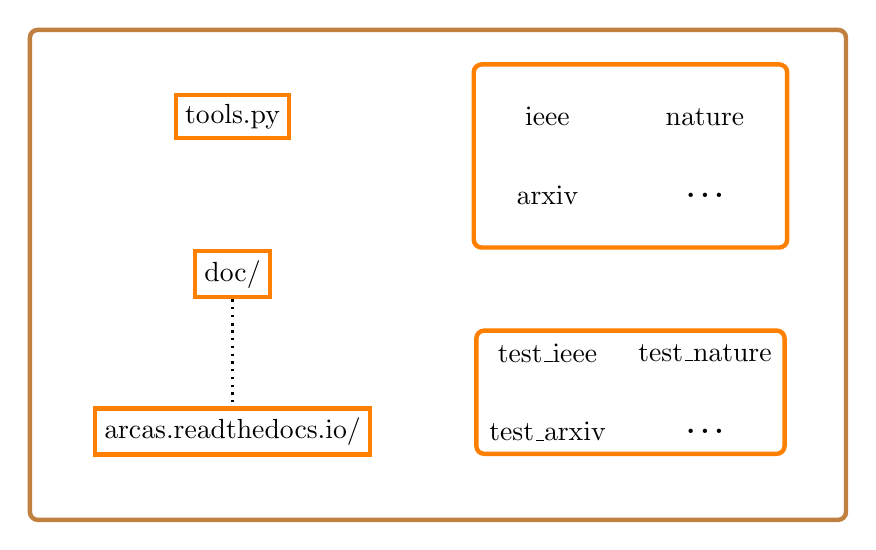
\begin{tikzpicture}

\tikzstyle{state}=[minimum width=0.4cm, font=\boldmath];
    

    \node[ultra thick, draw=orange] (0) at (0, 0) [state] {tools.py};
    \node[ultra thick, draw=orange] (1) at (0, -2) [state] {doc/};

    \node[ultra thick, draw=orange] (2) at (0, -4) [state] {arcas.readthedocs.io/};

    \node[ultra thick] (3) at (4, 0) [state] {ieee};
    \node[ultra thick] (4) at (6, 0) [state] {nature};
    \node[ultra thick] (5) at (4, -1) [state] {arxiv};
    \node[ultra thick] (6) at (6, -1) [state] {$\dots$};  

    \node [background, inner sep=4mm, fit=(3) (4) (5) (6)] {};

    \node[ultra thick] (7) at (4, -3) [state] {test{\_}ieee};
    \node[ultra thick] (8) at (6, -3) [state] {test{\_}nature};
    \node[ultra thick] (9) at (4, -4) [state] {test{\_}arxiv};
    \node[ultra thick] (10) at (6, -4) [state] {$\dots$};  

    \node [background, fit=(7) (8) (9) (10)] {};

    \draw (1) edge[out=-90, in=90, -, thick, dotted] node [above] {} (2);

    \node [background, brown, inner sep=8mm, fit= (0) (1) (2) (3) (4) (5) (6) (7) (8) (9) (10)] {};

\end{tikzpicture}
\end{document}